\documentclass{standalone}
\usepackage{tikz}
\usepackage{ctex,siunitx}
\setCJKmainfont{Noto Serif CJK SC}
\usepackage{tkz-euclide}
\usepackage{amsmath}
\usetikzlibrary{patterns, calc,3d}
\usetikzlibrary {decorations.pathmorphing,decorations.pathreplacing,decorations.shapes}
\begin{document}
\small
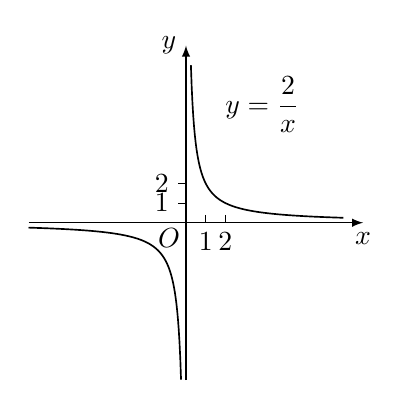
\begin{tikzpicture}[>=latex,scale=0.25]
  \draw[->](-8,0)--(9,0)node[below]{$x$};
  \draw[->](0,-8)--(0,9)node[left]{$y$};
  \draw[semithick,samples=200,domain=0.25:8]plot(\x,2/\x);
  \draw[semithick,samples=200,domain=-8:-0.25]plot(\x,2/\x);
  \foreach \x in {1,2} 
  {
    \draw[very thin](\x,0.4)--(\x,0)node[below]{$\x$};
    \draw[very thin](0,\x)--(-0.4,\x)node[left]{$\x$};
  }
  \node at (0,0)[below left,inner sep=2pt]{$O$};
  \node at (1.5,6)[right]{$y=\dfrac{2}{x}$};
\end{tikzpicture}
\end{document}